% !TEX root = ../main.tex
\newpage
\section{Hebbian Learning and Synaptic Plasticity}
\vspace{1mm}
\begin{quote}
\textsl{When an axon of cell A is near enough to excite a cell B and repeatedly or persistently takes part in firing it, some growth process or metabolic change takes places in one or both cells such that A's efficiency, as one of the cells firing B, is increased.}\cite{Hebb1949}
\end{quote}

This quote from Hebb has influenced the neuroscientific community since 1949. In its essence, Hebb postulated that neurons that \textsl{fire together, wire together}. It has since become known as \textsl{Hebbian learning}, and is simply modelled as a positive correlation between the action potentials of spiking neurons. It has been proven in vivo in many studies \cite{ChrolCannon2014}, just like its counterpart, \textsl{anti-Hebbian learning}, where a negative correlation can be found.


\subsection{Spike-timing dependant plasticity}
One specific temporal interpretation of these ideas is \textsl{spike-timing-dependent plasticity} (\STDP), where the relative timing of action potentials from the pre- and postsynaptic neuron determine causality \cite{Kempter1999, Gerstner2002}. If the postsynaptic neuron fires right after the presynaptic neuron, then we can expect the synaptic strength from post- to presynaptic neuron to increase, and vice versa. 

Let us say that neuron $\theta_i$ spikes at time $t_i$ and that neuron $\theta_j$ spikes at $t_j$. Taking the time difference $\Delta t_{ij}$ as $t_j - t_i$, we can say that when $\Delta t_{ij} > 0$ the spikes are correlated (there exists a temporally causal relation), and we can model an increase in synaptic strength of the connection from $\theta_i$ to $\theta_j$, which we will gather in the \textsl{coupling matrix} $K_{ij}$. In the same fashion we can decrease $K_{ji}$ when $\Delta t_{ij} < 0$ as there is no causal relation. \\

We can think of the coupling matrix as the continuous interpretation of $\kappa A_{ij}$, where synaptic strength and network topology go hand in hand. This also means that we need to redefine some concepts:
\begin{alignat}{2}
\kinbi &= \sum_{j=1}^{N} \rvert K_{i j} \rvert &&\koutbj = \sum_{i=1}^{N} \rvert K_{i j} \rvert \label{eq:definekinkoutfromK} \\
\kmean &= \frac{1}{N} \sum_{i,j=1}^{N} \rvert K_{i j} \rvert \hspace{15mm} && \: \:\hat{\kmean} = \frac{1}{N} \sum_{i,j=1}^{N} K_{i j}  \label{eq:kmeanfromK} 
\end{alignat}
The absolute value ensures that we capture the magnitude of the coupling strength. The reason we want to distinguish between $\kmean$ and $\hat{\kmean}$ is that for some parts of the investigation it is beneficial to study how inhibitive and excitatory coupling strengths influence each other.\\

The functions $W(t)$ that relate $\Delta t_{ij}$ to $\Delta K_{ij}$ are called \textsl{learning windows},  as they define a range in which $K_{ij}$ is able to adapt or \textsl{learn}, and also when learning is optimal. When signals between neurons show a very large time difference (negative or positive) we do not expect them to be correlated. Because the learning windows are generally not symmetrical we can also expect the coupling matrix to be asymmetrical.


%The magnitude of change is modulated by an asymmetric biphasic learning window around pulses originating from the postsynaptic neuron. Asymmetric because the peak is not situated at 0 and the integral over the window is generally positive, biphasic because this allows both to strengthen and weaken coupling strengths \cite{Gerstner2002}. 


This approach simplifies modeling the neuronal back-propagation, where another pulse is generated as an echo of the action potential which travels through the neuron dendrites (so, backwards). This behavior is believed to adjust the presynaptic weights, though it is a controversial subject \cite{Gerstner2002}. \\

In recent years, criticism on \STDP has been growing, as experimental data has shown that \STDP is usually accompanied by homeostatic plasticity of the neuron excitability and the synaptic strengths. Processes like \textsl{intrinsic plasticity} (\IP), where one neuron's excitability changes over time as to self-regulate sensitivity to incoming action potentials, or \textsl{synaptic scaling}, where synapse characteristics are adjusted in unison to counteract positive feedback loops, have proven to stabilize the firing rate \cite{ChrolCannon2014, Kirkwood2019}. When \STDP and \IP are combined, it seems like 
%We can model intrinsic plasticity by adjusting the neuron's excitability as the inverse of the firing rate: he more spikes that a neuron will receive, the less affected it is \cite{Song2017}.  An observed phenomenon is that the excitability evolves together with the coupling strength, but that at the extremes this relation reverses \cite{Debanne2017, Debanne2018}.  These types of plasticities should be relatively easy to implement but have no impact on the network topology.


\subsection{Formulation of \STDP as a model}
Following the notation in \cite{Kempter1999}, we will denote the spike train coming from each neuron $\theta_i$ as $S_i^{\rm out}(t) = \sum_{n} \delta (t-t_{i}^{n})$, where $t_{i}^{n}$ is the time that $\theta_i$ has fired. Similarly, we will denote the spike train coming into each neuron $\theta_i$ as $S_i^{\rm in}(t) = \sum_{f} \delta (t-t_{i}^{f})$. Now we can say that the synaptic strengths are adjusted as:
\begin{align}
\Delta K_{ij} &= \int_{t}^{t+\mathcal{T}} w^{\rm{out}} S_i^{\rm out}(\tau) + w^{\rm{in}} S_{j}^{\rm {in}}(\tau) \mathrm{d}\tau
+ \iint_{t}^{t+\mathcal{T}} W( \tau^\prime - \tau) S_{i}^{\rm out}(\tau) S_{j}^{\rm in}( \tau^\prime) \mathrm{d} \tau \mathrm{d} \tau^\prime
\label{eq:KempterSTDPFormulation1} \\
&= \sum_{t_i^{n}\in \mathcal{T}} w^{\mathrm{out}} + \sum_{t_{j}^{f} \in \mathcal{T}} w^{\mathrm{in}} + \sum_{t_{j}^{f}, t_i^{n} \in \mathcal{T}} W (t_{j}^{f}-t_i^{n} ) \label{eq:KempterSTDPFormulation2}
\end{align}


\subsection{Learning windows}
Another characteristic is the integral over the learning window. A window with a negative integral directs synaptic strengths mostly towards inhibitory behaviour, and vice versa with a positive integral. An integral of zero would mean that both inhibitory and excitatory synapses are stimulated equally. It has been proven that $\int W(\tau) \mathop{d\tau}$ is the correlation between signals \cite{Gerstner2002}. \\

Recently, triphasic learning windows have been used to account for when it takes too long for the postsynaptic neuron to fire, and thus to decorrelate the relation between neurons. These learning windows are curves that were fitted to experimental data of the cortex and the hippocampus \cite{ChrolCannon2014}.

The learning windows generally have $W(t^{\ast}) = 0$ for $t^{\ast} > 0$. This means that no learning will take place when the delay between neuron spikes is exactly $t^{\ast} > 0$. The triphasic windows show two of those points.

\subsubsection{Biphasic learning windows}
where \cite{Kempter1999} proposes the following learning window:
\begin{align}
W(t)_K = \alpha
\begin{cases}
\left[A_{p}\left(1-\frac{t}{\tilde{\tau}_{p}}\right)+A_{n}\left(1-\frac{t}{\tilde{\tau}_{n}}\right)\right] \cdot \exp \left( \frac{t}{\tau_{\rm syn}} \right) & \text{for } t \leq 0 \\
A_{p} \cdot \exp \left(-\frac{t}{\tau_{p}}\right) + A_{n} \cdot \exp \left(-\frac{t}{\tau_{n}} \right) & \text{for } t > 0
\end{cases} \label{eq:learningwindowKempter1999}
\end{align}
Here $t$ is the delay between presynaptic spike arrival and postsynaptic firing, $\alpha$ is a small learning parameter and all $\tau$ are time constants. Numerical values are usually  $\alpha = 0.05$, $\tau_{\rm syn} = 5$ ms, $\tau_{p} = 1$ ms, $\tau_{n} = 20$ ms and $A_p = 1$ and $A_{n} = -1$. $\tilde{\tau}_{p} \equiv \tau_{\rm syn} \tau_{p} / (\tau_{\rm syn} + \tau_{p})$ and $\tilde{\tau}_{n} \equiv \tau_{\rm syn} \tau_{n} / (\tau_{\rm syn} + \tau_{n})$. \\
$\int W(s)_K \mathrm{d}s = 2.56 \times 10^{-4}$.

\subsubsection{Song 2000}
The first formulation of \STDP as a mathematical model was in \cite{Song2000}. It is postulated without being concerned about the biological aspect too much. The synaptic strengths are simply updated as:
\begin{align}
\Delta K_{ij} &= K_{ij} \sum_{t_{j}^{f}, t_i^{n} \in \mathcal{T}} W (t_{j}^{f}-t_i^{n} ) \label{eq:SongSTDPFormulation}
\end{align}
The learning window is defined as a discontinuous function:
\begin{align}
W(t)_S =
\begin{cases}
A_{p} \cdot \exp \left(\frac{-t}{\tau_p}\right) & \text{for } s > 0 \\
A_{n} \cdot \exp \left(\frac{t}{\tau_n}\right)  & \text{for } s \leq 0
\end{cases} \label{eq:learningwindowKempter1999}
\end{align}
where we will use $A_p = 0.005$, $A_n = -0.00525$ and $\tau_p = \tau_n = 20$ ms. $\int W(s)_S \mathrm{d}s = -3.70 \times 10^{-4}$ so we expect the weights to be suppressed towards a negative value.

\begin{figure}[H]
\centering
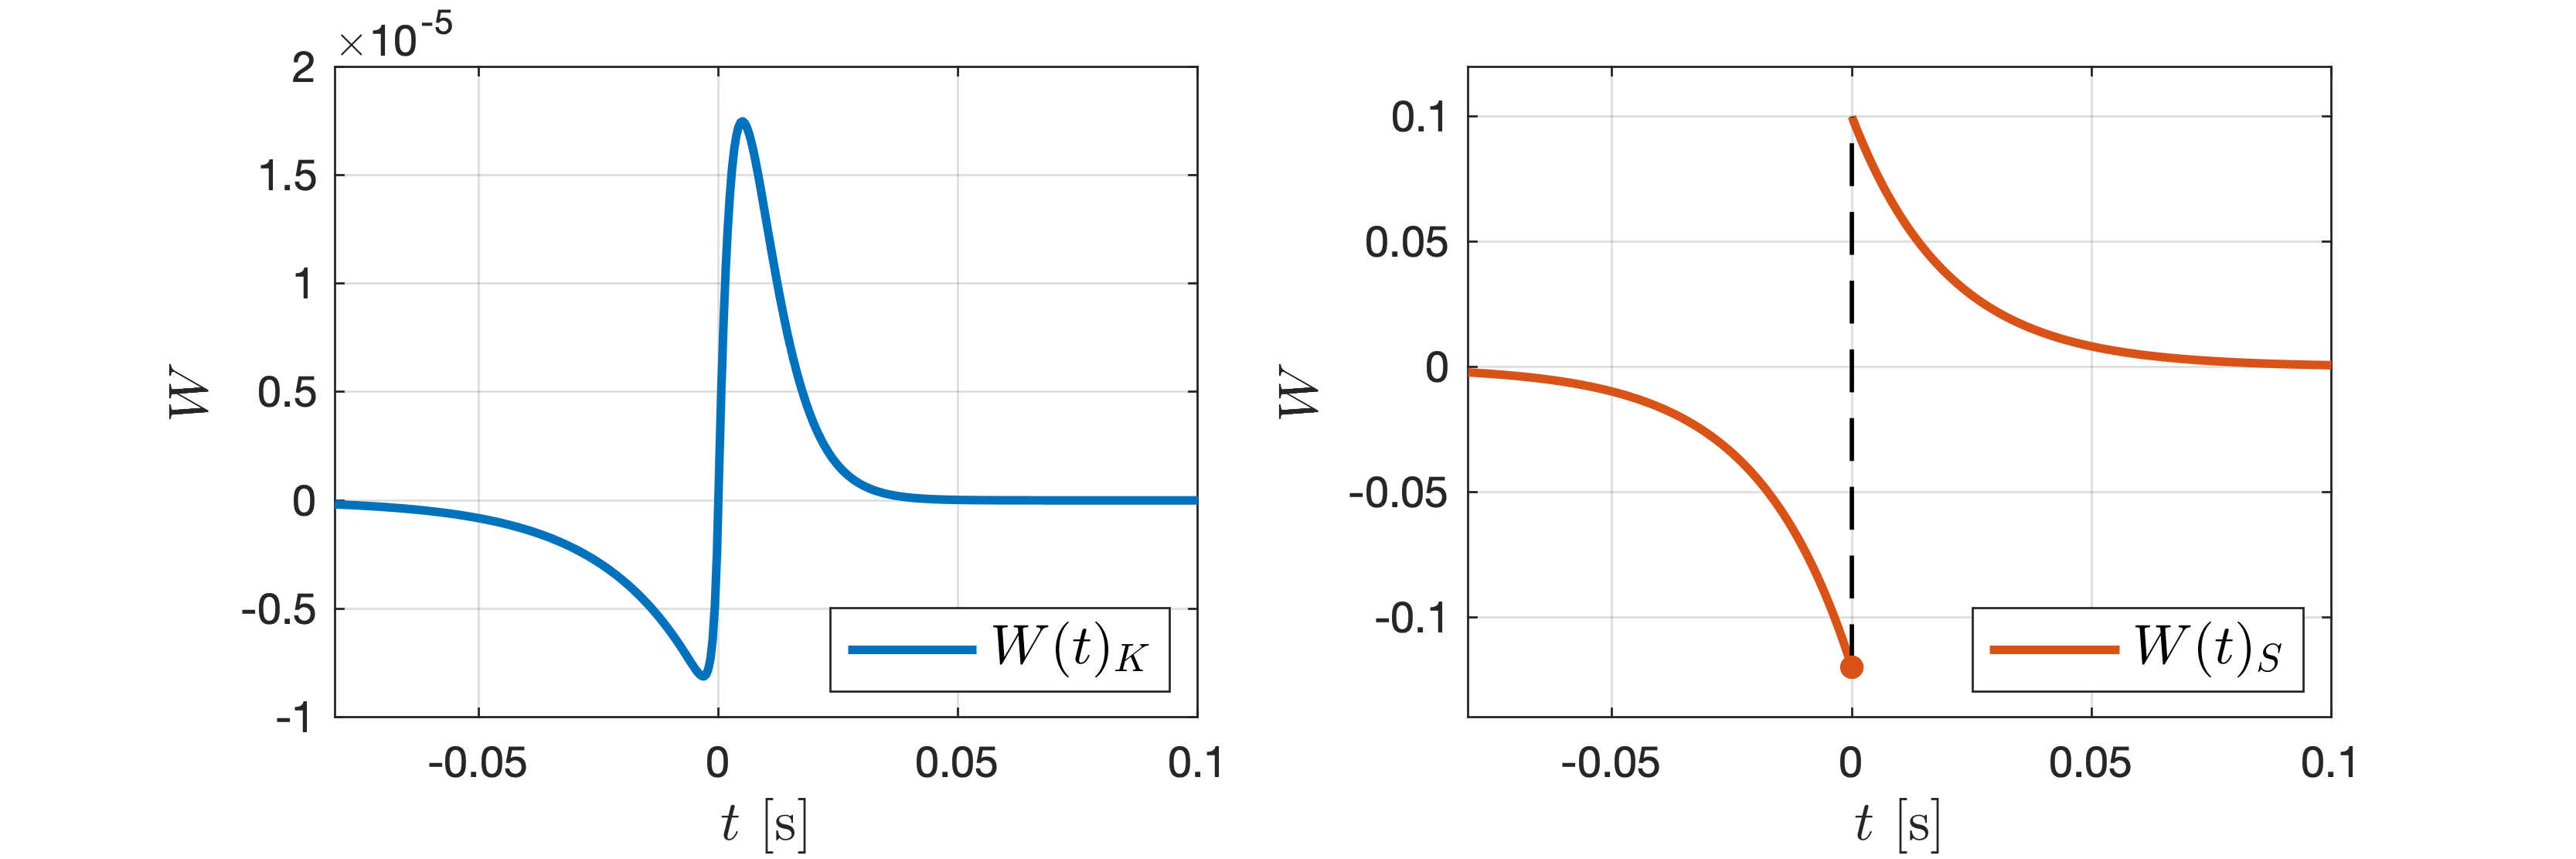
\includegraphics[width = \textwidth]{../Figures/LearningWindowsBiphasic.png}
\caption{Two different biphasic learning windows. We can see how in $W(t)_s$ a larger weight is put on the anti-Hebbian learning.}
\label{fig:LearningWindowsBiphasic}
\end{figure}


\subsection{Synaptic scaling}
There is no upper or lower bound on the synapse strength. Also generally, connection strengths are nonzero. This means that the notion of a \textsl{network} is lost.\\
One technique we can apply to keep the strengths within a definitive range is to scale homeostatically - a method where increases in synaptic strength will balance out any decreases by scaling:
\begin{align}
K_{ij}^s = K_{ij} \frac{\frac{1}{N} \sum_{i,j} K_{ij}}{\sum_{i} K_{ij}}
\end{align}
In this way, the out-degrees will remain constant. Using this approach, something has to remain constant, whether that is $\kmean$, or $\kmean^2$ or any other property of the adjacency matrix.


\subsection{Intrinsic plasticity}
Instead of scaling the weights to preserve a certain quantity in the network, we can allow the neurons to adjust the sensitivity to incoming signals. So when some synaptic strengths are increased, we can reduce the excitability. In \cite{Song2017} such a method is introduced in detail. We can simply update $\eta_{i} \rightarrow \eta_{i} + \eta_{\max } \cdot \phi_{i}$ where 
\begin{align}
\phi_{i} (t) =\left\{\begin{array}{l}-\alpha \cdot \exp \left(\frac{T_{\min }-t}{T_{\rm min }}\right) \text { if } t<T_{ \rm min } \\ \alpha \cdot \exp \left(\frac{t-T_{\rm max }}{T_{\max }}\right) \text { if } t >T_{\rm max } \\ 0, \text { otherwise }\end{array}\right.
\end{align}

\begin{figure}[H]
\centering
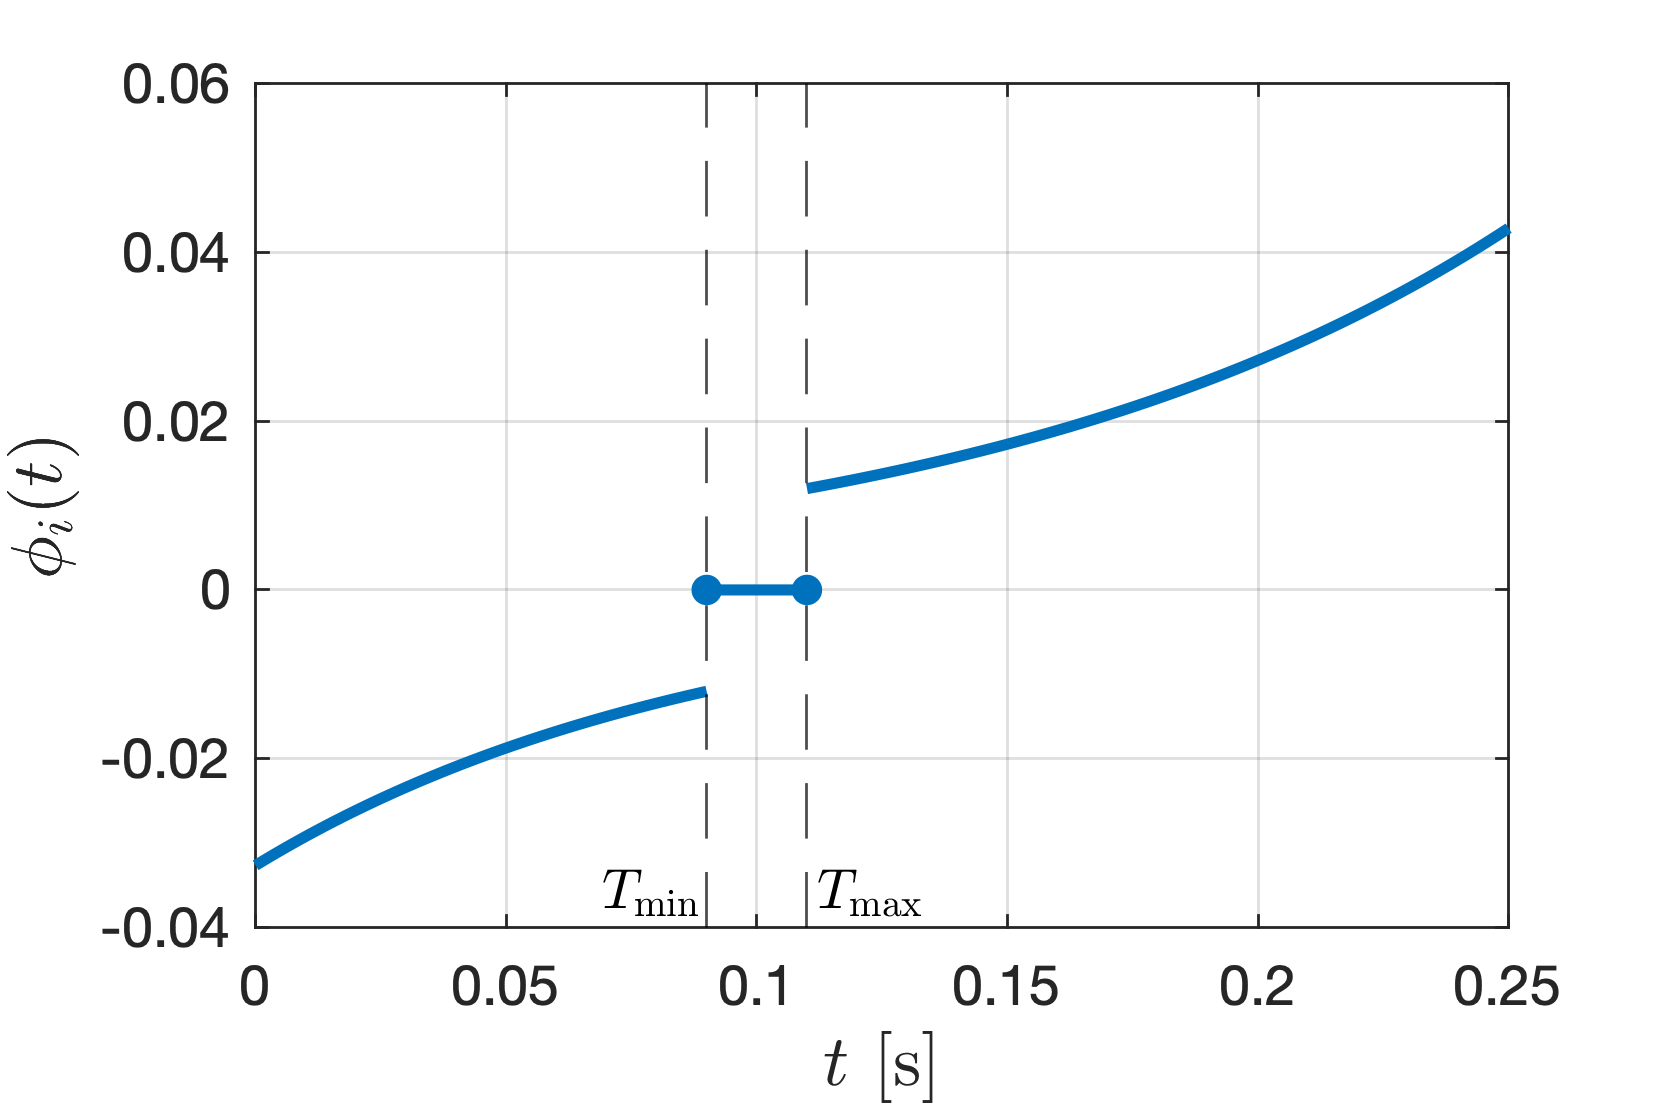
\includegraphics[width = 0.5\textwidth]{../Figures/Learning/IPlearningFunction.png}
\caption{The learning behaviour for the intrinsic plastiity.}
\label{fig:IPlearningFunction}
\end{figure}

